\documentclass[ignorenonframetext,]{beamer}
\setbeamertemplate{caption}[numbered]
\setbeamertemplate{caption label separator}{: }
\setbeamercolor{caption name}{fg=normal text.fg}
\beamertemplatenavigationsymbolsempty
\usepackage{lmodern}
\usepackage{amssymb,amsmath}
\usepackage{ifxetex,ifluatex}
\usepackage{fixltx2e} % provides \textsubscript
\ifnum 0\ifxetex 1\fi\ifluatex 1\fi=0 % if pdftex
  \usepackage[T1]{fontenc}
  \usepackage[utf8]{inputenc}
\else % if luatex or xelatex
  \ifxetex
    \usepackage{mathspec}
  \else
    \usepackage{fontspec}
  \fi
  \defaultfontfeatures{Ligatures=TeX,Scale=MatchLowercase}
\fi
\usetheme[]{Berlin}
% use upquote if available, for straight quotes in verbatim environments
\IfFileExists{upquote.sty}{\usepackage{upquote}}{}
% use microtype if available
\IfFileExists{microtype.sty}{%
\usepackage{microtype}
\UseMicrotypeSet[protrusion]{basicmath} % disable protrusion for tt fonts
}{}
\newif\ifbibliography
\hypersetup{
            pdftitle={Strategic Decision Making in the 3D Printing Industry - A Robust Decision Making (RDM) analysis},
            pdfauthor={Pedro Nascimento de Lima},
            pdfborder={0 0 0},
            breaklinks=true}
\urlstyle{same}  % don't use monospace font for urls
\usepackage{color}
\usepackage{fancyvrb}
\newcommand{\VerbBar}{|}
\newcommand{\VERB}{\Verb[commandchars=\\\{\}]}
\DefineVerbatimEnvironment{Highlighting}{Verbatim}{commandchars=\\\{\}}
% Add ',fontsize=\small' for more characters per line
\usepackage{framed}
\definecolor{shadecolor}{RGB}{248,248,248}
\newenvironment{Shaded}{\begin{snugshade}}{\end{snugshade}}
\newcommand{\KeywordTok}[1]{\textcolor[rgb]{0.13,0.29,0.53}{\textbf{#1}}}
\newcommand{\DataTypeTok}[1]{\textcolor[rgb]{0.13,0.29,0.53}{#1}}
\newcommand{\DecValTok}[1]{\textcolor[rgb]{0.00,0.00,0.81}{#1}}
\newcommand{\BaseNTok}[1]{\textcolor[rgb]{0.00,0.00,0.81}{#1}}
\newcommand{\FloatTok}[1]{\textcolor[rgb]{0.00,0.00,0.81}{#1}}
\newcommand{\ConstantTok}[1]{\textcolor[rgb]{0.00,0.00,0.00}{#1}}
\newcommand{\CharTok}[1]{\textcolor[rgb]{0.31,0.60,0.02}{#1}}
\newcommand{\SpecialCharTok}[1]{\textcolor[rgb]{0.00,0.00,0.00}{#1}}
\newcommand{\StringTok}[1]{\textcolor[rgb]{0.31,0.60,0.02}{#1}}
\newcommand{\VerbatimStringTok}[1]{\textcolor[rgb]{0.31,0.60,0.02}{#1}}
\newcommand{\SpecialStringTok}[1]{\textcolor[rgb]{0.31,0.60,0.02}{#1}}
\newcommand{\ImportTok}[1]{#1}
\newcommand{\CommentTok}[1]{\textcolor[rgb]{0.56,0.35,0.01}{\textit{#1}}}
\newcommand{\DocumentationTok}[1]{\textcolor[rgb]{0.56,0.35,0.01}{\textbf{\textit{#1}}}}
\newcommand{\AnnotationTok}[1]{\textcolor[rgb]{0.56,0.35,0.01}{\textbf{\textit{#1}}}}
\newcommand{\CommentVarTok}[1]{\textcolor[rgb]{0.56,0.35,0.01}{\textbf{\textit{#1}}}}
\newcommand{\OtherTok}[1]{\textcolor[rgb]{0.56,0.35,0.01}{#1}}
\newcommand{\FunctionTok}[1]{\textcolor[rgb]{0.00,0.00,0.00}{#1}}
\newcommand{\VariableTok}[1]{\textcolor[rgb]{0.00,0.00,0.00}{#1}}
\newcommand{\ControlFlowTok}[1]{\textcolor[rgb]{0.13,0.29,0.53}{\textbf{#1}}}
\newcommand{\OperatorTok}[1]{\textcolor[rgb]{0.81,0.36,0.00}{\textbf{#1}}}
\newcommand{\BuiltInTok}[1]{#1}
\newcommand{\ExtensionTok}[1]{#1}
\newcommand{\PreprocessorTok}[1]{\textcolor[rgb]{0.56,0.35,0.01}{\textit{#1}}}
\newcommand{\AttributeTok}[1]{\textcolor[rgb]{0.77,0.63,0.00}{#1}}
\newcommand{\RegionMarkerTok}[1]{#1}
\newcommand{\InformationTok}[1]{\textcolor[rgb]{0.56,0.35,0.01}{\textbf{\textit{#1}}}}
\newcommand{\WarningTok}[1]{\textcolor[rgb]{0.56,0.35,0.01}{\textbf{\textit{#1}}}}
\newcommand{\AlertTok}[1]{\textcolor[rgb]{0.94,0.16,0.16}{#1}}
\newcommand{\ErrorTok}[1]{\textcolor[rgb]{0.64,0.00,0.00}{\textbf{#1}}}
\newcommand{\NormalTok}[1]{#1}
\usepackage{longtable,booktabs}
\usepackage{caption}
% These lines are needed to make table captions work with longtable:
\makeatletter
\def\fnum@table{\tablename~\thetable}
\makeatother
\usepackage{graphicx,grffile}
\makeatletter
\def\maxwidth{\ifdim\Gin@nat@width>\linewidth\linewidth\else\Gin@nat@width\fi}
\def\maxheight{\ifdim\Gin@nat@height>\textheight0.8\textheight\else\Gin@nat@height\fi}
\makeatother
% Scale images if necessary, so that they will not overflow the page
% margins by default, and it is still possible to overwrite the defaults
% using explicit options in \includegraphics[width, height, ...]{}
\setkeys{Gin}{width=\maxwidth,height=\maxheight,keepaspectratio}

% Prevent slide breaks in the middle of a paragraph:
\widowpenalties 1 10000
\raggedbottom

\AtBeginPart{
  \let\insertpartnumber\relax
  \let\partname\relax
  \frame{\partpage}
}
\AtBeginSection{
  \ifbibliography
  \else
    \let\insertsectionnumber\relax
    \let\sectionname\relax
    \frame{\sectionpage}
  \fi
}
\AtBeginSubsection{
  \let\insertsubsectionnumber\relax
  \let\subsectionname\relax
  \frame{\subsectionpage}
}

\setlength{\parindent}{0pt}
\setlength{\parskip}{6pt plus 2pt minus 1pt}
\setlength{\emergencystretch}{3em}  % prevent overfull lines
\providecommand{\tightlist}{%
  \setlength{\itemsep}{0pt}\setlength{\parskip}{0pt}}
\setcounter{secnumdepth}{0}

\title{Strategic Decision Making in the 3D Printing Industry - A Robust
Decision Making (RDM) analysis}
\author{Pedro Nascimento de Lima}
\date{25 de setembro de 2018}

\begin{document}
\frame{\titlepage}

\begin{frame}
\tableofcontents[hideallsubsections]
\end{frame}

\section{Why 3D Printing}\label{why-3d-printing}

\begin{frame}{Key Features of 3D printing}

\begin{itemize}
\tightlist
\item
  3D printing may
\end{itemize}

\end{frame}

\begin{frame}{Why 3D Printing?}

3D Printing is an emergint technology, but decision makers face
uncertainty.

\begin{block}{Positive Evidence}

\begin{itemize}
\tightlist
\item
  3D printing Industry has seen two digits growth consistently in the
  last few years;
\item
  3D printing is already reshaping supply chains across industries
  (e.g.: prothesis, aerospace, etc.);
\end{itemize}

\end{block}

\begin{block}{Negative Evidence}

\begin{itemize}
\tightlist
\item
  Major players have been observing declining profitability (e.g.:
  Stratasys, 3D Systems);
\item
  Estimates of 3D printing growth diverge;
\end{itemize}

\end{block}

\end{frame}

\begin{frame}{3D Printing Prospected Effects - Why do we Care?}

\end{frame}

\begin{frame}{Shaping events in the 3D Printing Industry}

\begin{itemize}
\tightlist
\item
  Patent Dynamics
\end{itemize}

\begin{block}{Patent Dynamics and Expiration}

The FDM patent expiration in 2007

\end{block}

\begin{block}{Strategies Played by Key Players}

Leading 3D printing players (e.g.~3D Systems and Stratasys) historically
have been adopting a closed-source strategy.

However, the key event leading to 3D printing growth was patent
expiration.

\begin{block}{Dynamyc Hipothesis 1: Holding Patents m}

\end{block}

\end{block}

\begin{block}{A fourth level}

Some Text Here

\begin{block}{A fith level}

When you click the \textbf{Knit} button a document will be generated
that includes both content as well as the output of any embedded R code
chunks within the document.

\end{block}

\end{block}

\end{frame}

\subsection{Slide with Bullets}\label{slide-with-bullets}

\begin{itemize}
\tightlist
\item
  Bullet 1
\item
  Bullet 2
\item
  Bullet 3
\end{itemize}

\section{XLRM}\label{xlrm}

\subsection{Model}\label{model}

\begin{Shaded}
\begin{Highlighting}[]
\KeywordTok{summary}\NormalTok{(cars)}
\end{Highlighting}
\end{Shaded}

\begin{verbatim}
##      speed           dist       
##  Min.   : 4.0   Min.   :  2.00  
##  1st Qu.:12.0   1st Qu.: 26.00  
##  Median :15.0   Median : 36.00  
##  Mean   :15.4   Mean   : 42.98  
##  3rd Qu.:19.0   3rd Qu.: 56.00  
##  Max.   :25.0   Max.   :120.00
\end{verbatim}

\section{Case Generation}\label{case-generation}

\begin{frame}{Design of Experiments}

\begin{itemize}
\tightlist
\item
  Full factorial design of these variables, resulting in 54 strategies:
\end{itemize}

\begin{longtable}[]{@{}lll@{}}
\toprule
\begin{minipage}[b]{0.14\columnwidth}\raggedright\strut
Variable\strut
\end{minipage} & \begin{minipage}[b]{0.47\columnwidth}\raggedright\strut
Meaning\strut
\end{minipage} & \begin{minipage}[b]{0.30\columnwidth}\raggedright\strut
Levels\strut
\end{minipage}\tabularnewline
\midrule
\endhead
\begin{minipage}[t]{0.14\columnwidth}\raggedright\strut
\(S_1\)\strut
\end{minipage} & \begin{minipage}[t]{0.47\columnwidth}\raggedright\strut
Market \& Pricing Strategy. Defines wether the player pursue an
agressive marketing strategy to gain market share (by cutting prices and
accepting excess capacity), or pursue a conservative strategy,\strut
\end{minipage} & \begin{minipage}[t]{0.30\columnwidth}\raggedright\strut
Agressive (1); Conservative (2)\strut
\end{minipage}\tabularnewline
\begin{minipage}[t]{0.14\columnwidth}\raggedright\strut
\(S_1^{max}\) or \(S_1^{min}\)\strut
\end{minipage} & \begin{minipage}[t]{0.47\columnwidth}\raggedright\strut
Desired Market Share. For a Conservative Strategy, the player adopts the
\(S_1^{max}\), and for an Agressive Strategy, \(S_1^{min}\)\strut
\end{minipage} & \begin{minipage}[t]{0.30\columnwidth}\raggedright\strut
20\%; 30\%; 40\%\strut
\end{minipage}\tabularnewline
\begin{minipage}[t]{0.14\columnwidth}\raggedright\strut
\(\eta_1\)\strut
\end{minipage} & \begin{minipage}[t]{0.47\columnwidth}\raggedright\strut
R \& D budget, as a fraction of revenue.\strut
\end{minipage} & \begin{minipage}[t]{0.30\columnwidth}\raggedright\strut
5\%; 10\%; 15\%\strut
\end{minipage}\tabularnewline
\begin{minipage}[t]{0.14\columnwidth}\raggedright\strut
\(\kappa_i\)\strut
\end{minipage} & \begin{minipage}[t]{0.47\columnwidth}\raggedright\strut
Fraction of R \& D budget released to open source technologies.\strut
\end{minipage} & \begin{minipage}[t]{0.30\columnwidth}\raggedright\strut
0 \%; 50 \%; 90 \%\strut
\end{minipage}\tabularnewline
\bottomrule
\end{longtable}

\end{frame}

\begin{frame}{Candidate Strategy NPV across scenarios}

\begin{center}\includegraphics{dmdu-presentation_files/figure-beamer/unnamed-chunk-1-1} \end{center}

\end{frame}

\begin{frame}{Global Demand across scenarios}

\begin{center}\includegraphics{dmdu-presentation_files/figure-beamer/unnamed-chunk-2-1} \end{center}

\end{frame}

\begin{frame}{Market Share of the 4 Players in a given scenario}

\begin{center}\includegraphics{dmdu-presentation_files/figure-beamer/unnamed-chunk-3-1} \end{center}

\end{frame}

\begin{frame}{Net Present Value across strategies and Scenarios}

\begin{center}\includegraphics{dmdu-presentation_files/figure-beamer/unnamed-chunk-4-1} \end{center}

\end{frame}

\begin{frame}{Regret across strategies and Scenarios}

\begin{center}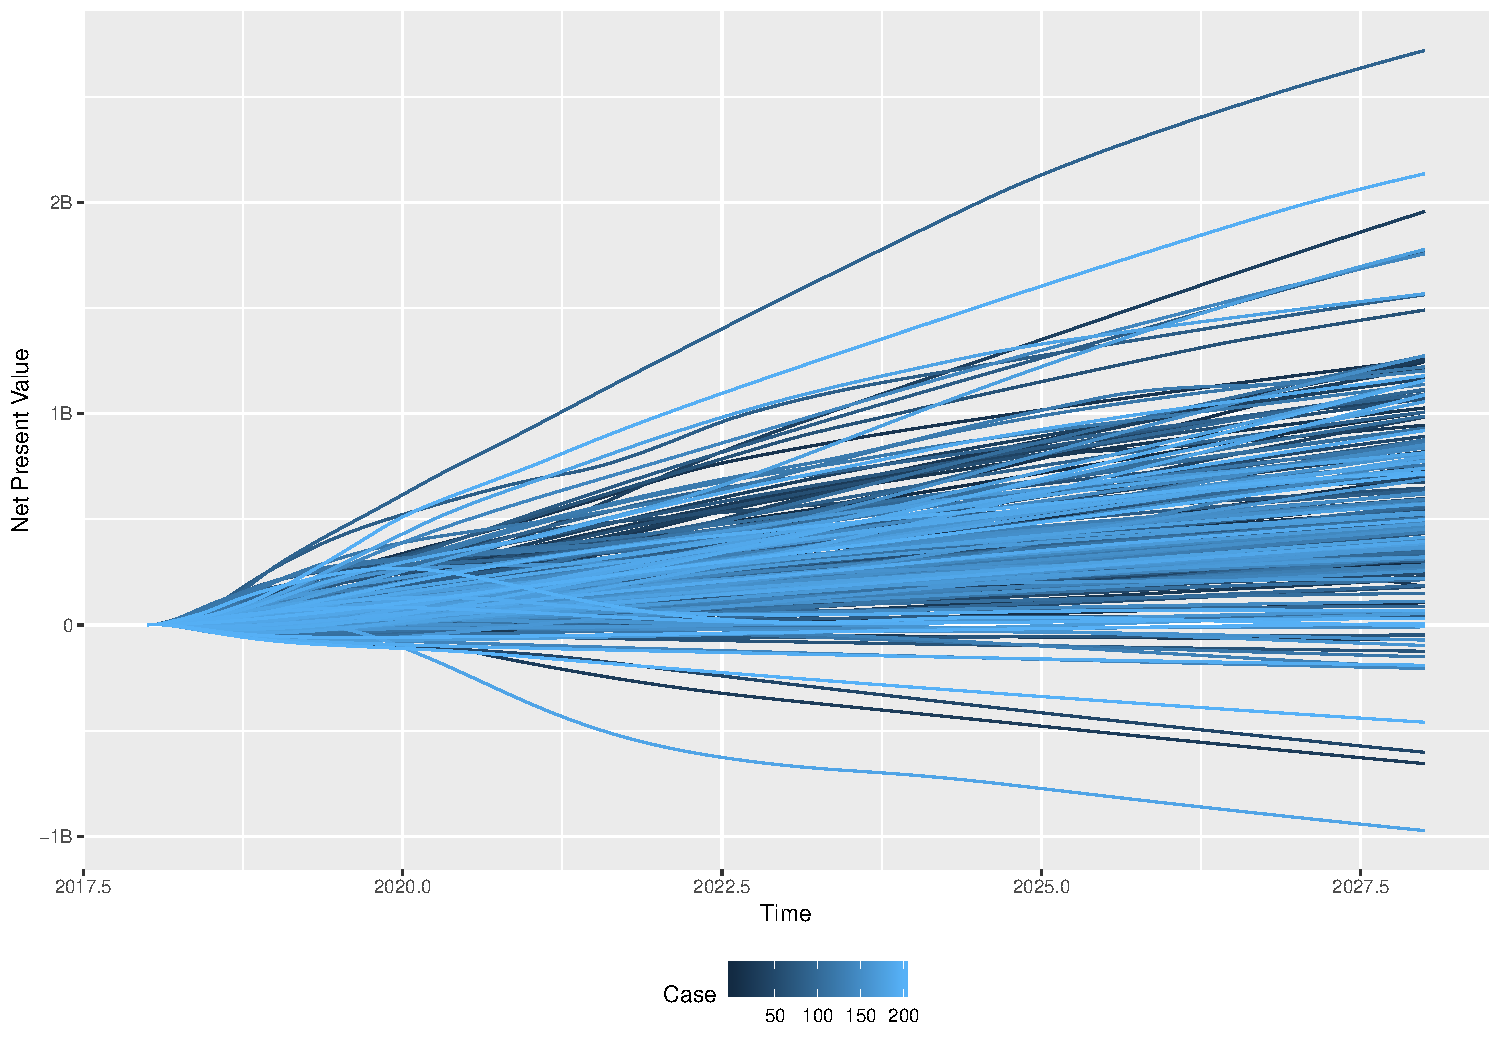
\includegraphics{dmdu-presentation_files/figure-beamer/unnamed-chunk-5-1} \end{center}

\end{frame}

\begin{frame}{Ranking Strategies by Regret}

\begin{table}[H]
\centering
\resizebox{\linewidth}{!}{
\begin{tabular}{rrrrr}
\toprule
Lever & Capac. Strategy & Desired Mkt Share & R\&D Inv. & Open Source R\&D\\
\midrule
19 & 0.3 & 0.05 & 0.0 & 217247495\\
31 & 0.4 & 0.05 & 0.0 & 261350277\\
25 & 0.2 & 0.05 & 0.0 & 261414542\\
13 & 0.4 & 0.10 & 0.0 & 327653642\\
1 & 0.3 & 0.10 & 0.0 & 332802086\\
\addlinespace
27 & 0.2 & 0.05 & 0.5 & 353242981\\
21 & 0.3 & 0.05 & 0.5 & 365209080\\
7 & 0.2 & 0.10 & 0.0 & 375355405\\
32 & 0.4 & 0.05 & 0.0 & 424089389\\
20 & 0.3 & 0.05 & 0.0 & 449632071\\
\bottomrule
\end{tabular}}
\end{table}

\end{frame}

\section{Scenario Discovery}\label{scenario-discovery}

\section{Tradeoffs}\label{tradeoffs}

\section{Second Iteration}\label{second-iteration}

\section{Final Thoughts}\label{final-thoughts}

\subsection{Slide with Plot}\label{slide-with-plot}

\includegraphics{dmdu-presentation_files/figure-beamer/pressure-1.pdf}

\end{document}
